\section{Wstęp}
Grafika komputerowa i gry komputerowe napędzają rozwój sprzętu
komputerowego. Jeszcze nie tak dawno gry 2D były hitem, dzisiaj każda szanująca
się gra jest osadzona w świecie 3D z niezwykle realistyczną grafiką. Świat we
współczesnych grach jest tak realistyczny, że czasami trudno jest już go
odróżnić od świata rzeczywistego. Zaawansowane technologie związane z grafiką
trójwymiarową są również wykorzystywane w innych dziedzinach np. kinematografii,
komputerowo wspomaganym projektowaniu, medycynie i wielu innych.

{
\addtocounter{footnote}{1}
\begin{figure}[h!]
  \centering
  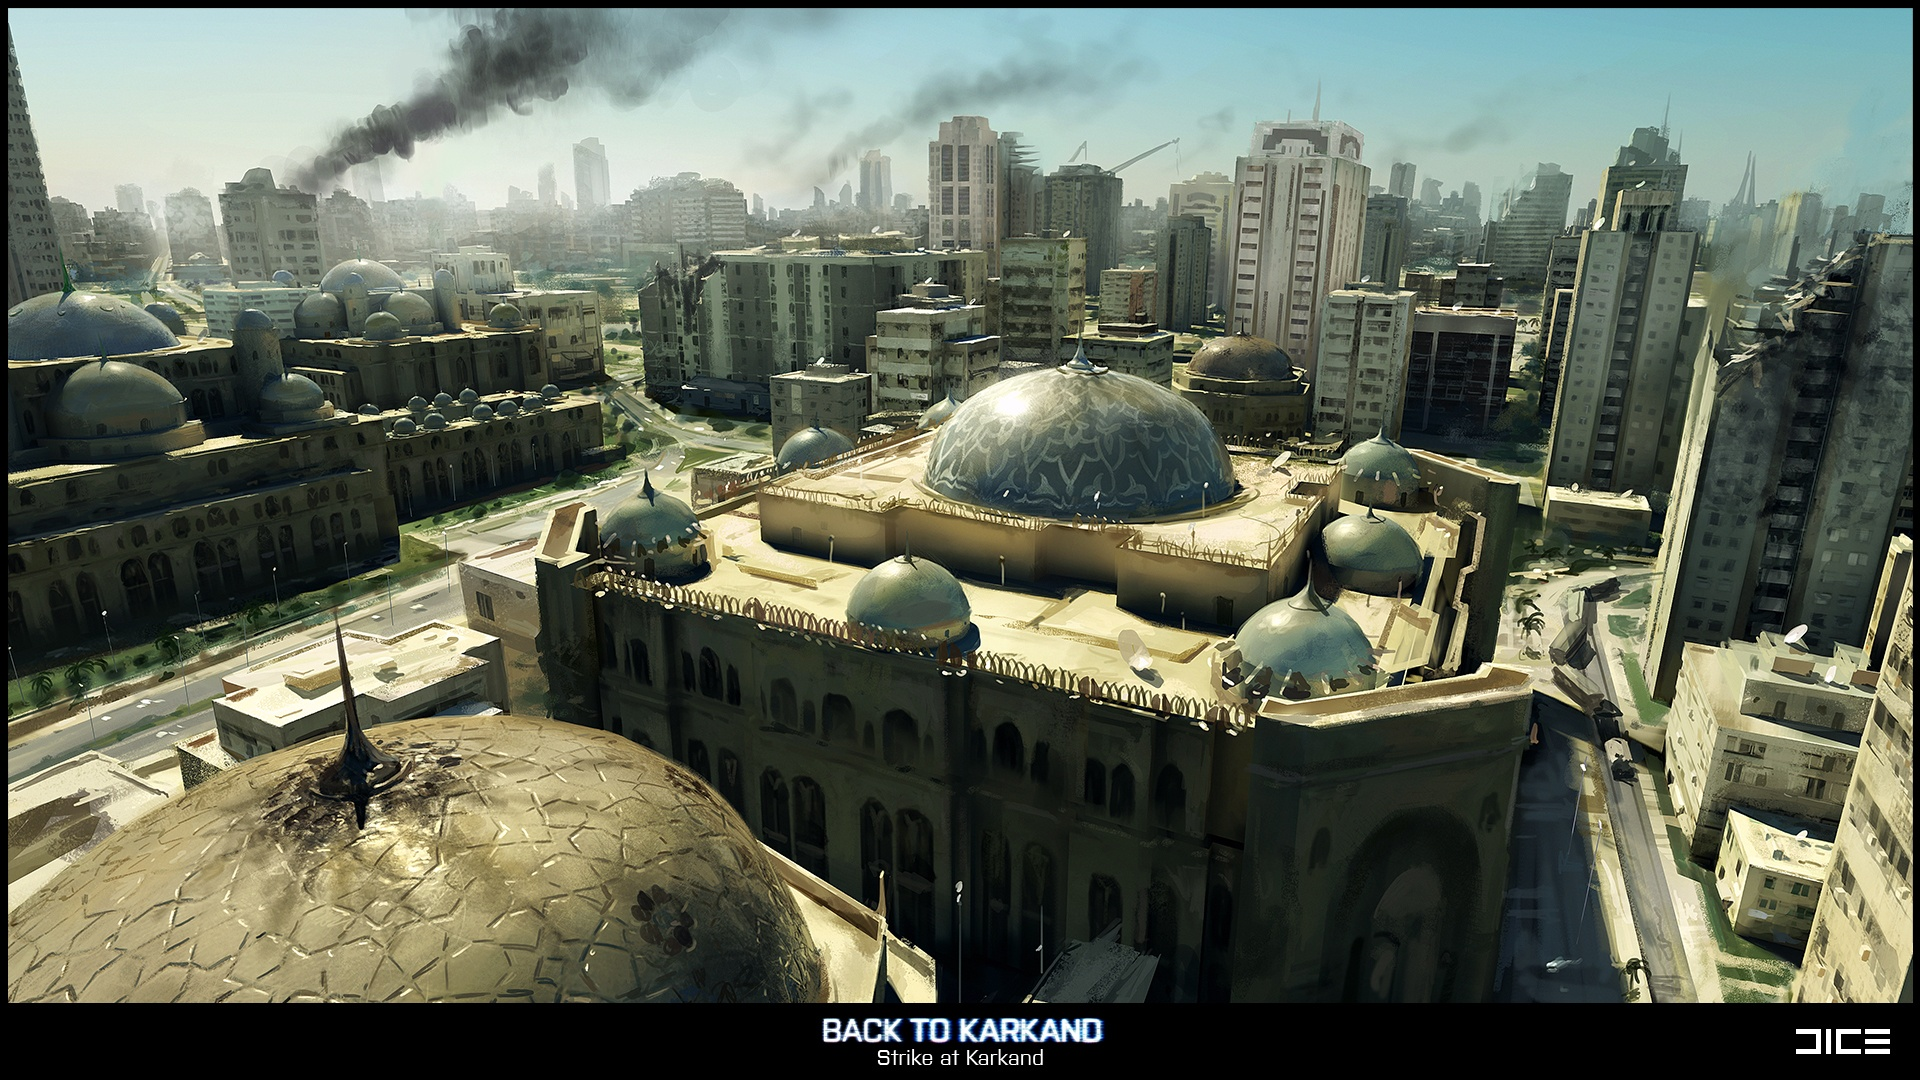
\includegraphics[width=0.8\textwidth]{images/bf3_1.jpg}
  \caption[Gra Battlefield 3]{Gra Battlefield 3~$^{\decimal{footnote}}$.}
\end{figure}
\begin{figure}[h!]
  \centering
  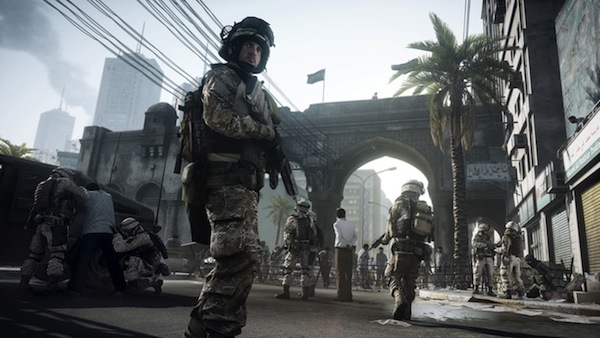
\includegraphics[width=0.8\textwidth]{images/bf3_2.jpg}
  \caption[Gra Battlefield 3 cd.]{Gra Battlefield 3~$^{\decimal{footnote}}$ cd.}
\end{figure}
\footnotetext[\value{footnote}]{\url{http://www.pcgamer.com/2011/05/11/battlefield-3-back-to-karkand-map-pack-detailed/}
%\url{http://www.g4tv.com/thefeed/blog/post/712382/battlefield-3-to-be-the-biggest-launch-in-eas-history/}
}
\addtocounter{footnote}{1}
\begin{figure}[h!]
  \centering
  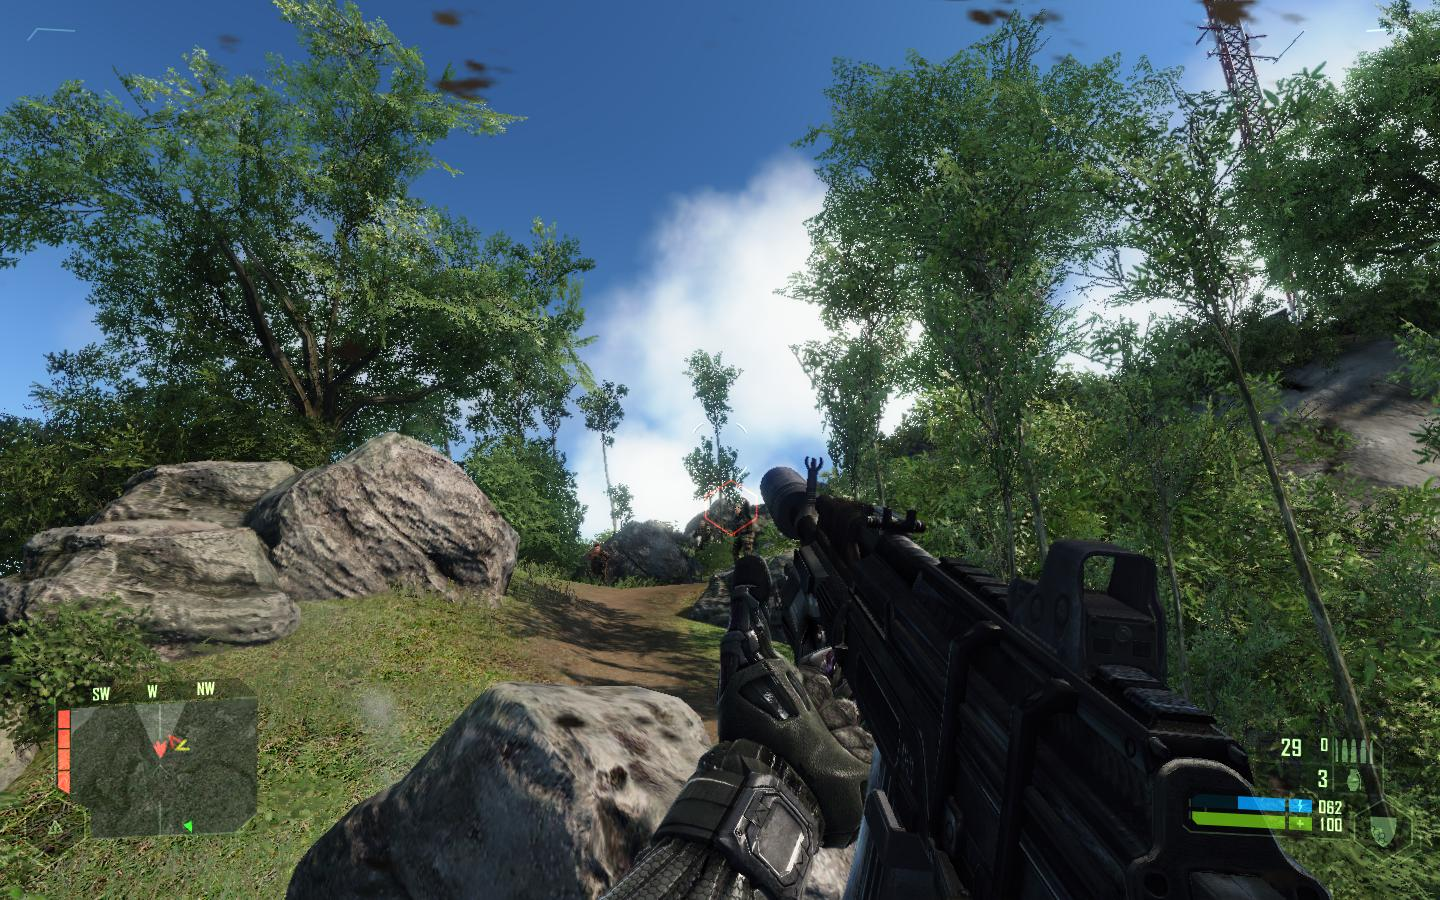
\includegraphics[width=0.8\textwidth]{images/Crysis2.JPG}
  \caption[Gra Crysis 2]{Gra Crysis 2~$^{\decimal{footnote}}$.}
\end{figure}
\footnotetext[\value{footnote}]{\url{http://mattplays.com/game/crysis/}}
}

Głównym problemem w dzisiejszych czasach nie jest stworzenie realistycznego
świata, a realistycznego człowieka. Jednym z ciekawszych projektów poruszających
ten temat jest program o nazwie Emily~\cite{link01}, gdzie rozpoznanie czy jest
to animacja 3D czy prawdziwy człowiek jest praktycznie niemożliwe.

Zastosowanie syntetycznego generowania obiektów 3D ma zastosowanie nie tylko w
grach komputerowych czy w kinematografii, ale również może zostać wykorzystane w
kompresji obrazu. Doszliśmy już do granicy możliwości kompresji obrazu z
wykorzystaniem transformacji
Fouriera~\footnote{\url{http://mathworld.wolfram.com/FourierTransform.html}}
czy transformacji
falkowej~\footnote{\url{http://mathworld.wolfram.com/WaveletTransform.html}}.
Dalszy rozwój w tym kierunku nie daje już dużego skoku na rozmiarze czy jakości
kompresowanego obrazu. Ograniczenie to wymusza nowe podejście do kompresji
obrazu polegające na syntezie obrazu do znanych wzorów, tak jak to robi nasz
mózg --- gdy oglądamy filmy nie musimy widzieć dokładnie jak układają się źdźbła
trawy --- informacja, że na scenie znajduje się trawa wystarczy, tak samo nie
interesuje nas ile jest chmur na niebie --- tylko to, że jest
zachmurzenie. Tak samo można skompresować obraz przedstawiający ludzką twarz ---
nie interesuje nas faktura skóry twarzy czy rozmieszczenie włosów na głowie
aktora, nawet niekiedy nie interesuje nas sam wygląd aktora jeśli go nie znamy,
interesuje nas zaś, w której scenie dany aktor występuje i co takiego robi/mówi.
Gdybyśmy więc kompresując film zapisywali ogólny wygląd aktora w postaci
parametrów modelu człowieka i w kolejnych klatkach animacji zmieniali tylko
parametry opisujące mimikę twarzy aktora mielibyśmy doskonałą kompresję --- a
jakość filmu zależałaby tylko od szczegółowości modelu obiektów.

Niniejsza praca skupia się głównie na twarzy ludzkiej, opisuje powierzchownie
jej budowę (kształt) oraz proponuje formę opisu twarzy (wiedza) w oparciu o
gramatykę kształtu.

W internecie jest dość niewiele aplikacji generujących twarz trójwymiarową na
podstawie zdjęć. Jedną z tych, które udało nam się znaleźć jest FaceGen firmy
Singular~\cite{link04}. Aplikacja ta jest bardziej nastawiona na edycje twarzy
(ruchy ust, ruchy powiek, mimika), generowanie twarzy na podstawie profili
jest tylko dodatkiem. Aplikacja potrafi nawet na podstawie zdjęć przygotować
odpowiednią teksturę, która po nałożeniu na model polepsza realizm twarzy.

Synteza twarzy ludzkiej jest młodą dziedziną, gdyż dopiero od niedawna sprzęt
komputerowy jest na tyle wydajny, by w rozsądnym czasie wygenerować obiekt.
Dość trudną sprawą w całym zadaniu jest analiza obrazu, rozpoznanie gdzie na
obrazie znajdują się punkty charakterystyczne twarzy takie jak oczy, usta czy
nos. Niniejsza praca nie będzie wgłębiała się w elementy lokalizowania
twarzy na zdjęciu czy wyszukiwaniu punktów charakterystycznych, na ten
temat jest mnóstwo materiałów w sieci (od metod gradientowych po analizę
koloru). Skupimy się głównie na ręcznym wyznaczeniu charakterystycznych
elementów twarzy, których wierne przeniesienie na model komputerowy będzie
kluczowe w celu wygenerowania twarzy trójwymiarowej. Drugim istotnym
zagadnieniem poruszonym w tej pracy jest przetransformowanie wiedzy uzyskanej w
poprzednim etapie na gramatykę kształtu twarzy. Po uzyskaniu punktów
charakterystycznych i mając opis twarzy za pomocą gramatyki kształtu bądź jej
prototyp, wygenerowanie obiektu nie powinno być kłopotliwe, oczywiście jeśli tą
wiedzę posiadamy. Zadanie to nie jest proste ze względu na skomplikowany
wygląd twarzy ludzkiej, praktycznie niewielka zmiana położenia oczu, nosa bądź
ust, całkowicie może zmienić wygląd twarzy.

\subsection{Cel i~zakres pracy}
Celem pracy jest opisanie skomplikowanej budowy twarzy ludzkiej i zaproponowanie
modelu jej opisu w postaci gramatyki kształtu, który wraz z informacją o
położeniu punktów charakterystycznych na obrazie wygeneruje obiekt 3D w pewnym
zakresie zbliżony do twarzy źródłowej. Będziemy się starać, aby model ten był na
tyle uniwersalny, by niewielkim nakładem pracy móc opisać nie tylko
twarz ale całe ciało ludzkie. Praktyczną częścią pracy będzie stworzenie
niewielkiej aplikacji wykorzystującej wyżej wspomniany model, która na
podstawie szkiców bądź zdjęć profili twarzy ludzkiej będzie generowała model 3D
twarzy. Przy odpowiednim zdefiniowaniu i sparametryzowaniu schematu zestaw
danych mógłby jednoznacznie identyfikować osobę. Mogłoby to być wykorzystywane w
rozpoznawaniu osób na podstawie profili. Rozszerzenie pracy o wyciąganie danych
z dowolnych zdjęć ułatwiłoby wyszukiwanie i identyfikację osoby w tłumie, na
podstawie szczątkowych danych z obrazu (twarz częściowo zasłonięta, lekko
obrócona).

\subsection{Streszczenie pracy}
Całość pracy jest podzielona na siedem rozdziałów, w których zawarto
odpowiednio:
\begin{itemize}
  \item rozdział 1 zawiera opis zagadnienia poruszanego w pracy;
  \item rozdział 2 zawiera opis metod przenoszenia obiektów do 3D;
  \item rozdział 3 zawiera wstęp teoretyczny do gramatyk kształtów;
  \item rozdział 4 zawiera opis spojrzenie na to jak ten problem rozwiązali
  inni;
  \item rozdział 5 zawiera opis koncepcji systemu, co~należy wykonać
  w~praktycznej części pracy;
  \item w rozdziale 6 znajduje się opis implementacji praktycznej części pracy;
  \item w rozdziale 7 znajdują się przykładowe symulacje, eksperymenty z
  aplikacją i ich wyniki;
  \item rozdział 8 zawiera podsumowanie pracy, co udało się wykonać, opis
  napotkanych trudności, jak można rozszerzyć dziedzinę projektu oraz uwagi
  końcowe.
\end{itemize}
